\documentclass[main.tex]{subfile}
\begin{document}

\section{Delopgave 1\\\normalsize{-- Multitrådet sum}}
Formålet med denne delopgave er at vise, at vi kan anvende (multiple) tråde til at foretage paralelle operationer, og på den måde udnytte multikerne hardware til at udføre beregningsopgaver hurtigere.

\subsection{Implementationen, overordnet set}
Med udgangspunkt i den udleverede kode (Silberschatz s.171) har vi konstrueret et program som kan beregne sumfunktionen.
\begin{equation*}
sum = \sum_{i=0}^N i.
\end{equation*}

Programmet tager 2 parametre: \textit{N} (øvre grænse for summeringen) og \textit{t} (antal tråde programmet skal starte).\\

Vi benytter en \textit{struct Sumjob} til at sende parametre til trådene.\\

Programmet udskriver resultatet til terminalen efter alle beregninger er foretaget.

\subsection{De specifikke løsninger}
I første omgang er det værd at nævne, at ændringerne til den udleverede kode har betydet, at kontrol programmet foretager af input også skulle ændres. Da programmet tager en ekstra parameter, og at denne parameter skal være et positivt heltal er reflekteret med en ekstra \texttt{if}-statement og en ændring ift. check af antal parametre.

\subsubsection{Sum med multitråd}
Da brugeren angiver antallet af tråde som inputparameter til programmet, er det nødvendigt at allokere hukommelse til trådenes id (\textit{pthread\_t}). Det er ligeledes nødvendigt at allokere hukommelse til de \textit{Sumjob} trådene starter. Både vores \textit{pthread\_t} og \textit{Sumjob} oprettes i arrays. Der beregnes desuden det interval af heltal, som hver tråd skal summere.\\ 

Ved at iterere (i en for-løkke) igennem vore \textit{Sumjob} sætter vi (baseret på intervallet) det første og sidste heltal som skal summeres af hver tråd, hvorefter vi starter metoden \textit{runner} i tråden med \textit{Sumjob}'et som parameter.\\

Herefter starter vi en ny for-løkke, hvori vi kalder \textit{pthread\_join} for hver tråd-id, hvormed vi afventer trådene bliver færdige. Til sidst frigiver vi (for en god ordens skyld) hukommelsen allokeret til tråde og jobs. Til sidst printer vi resultatet til terminalen.

\subsubsection{Sum af kvadratrod}
For at beregne summen af kvadratroden \textit{sumsqrt} er det nødvendigt at regne i flydende tal i stedet for heltal. Det betyder dog ingen forskel for trådene som sådan: metoden \textit{runner} som foretager summeringen arbejder med de samme input (intervallet), men benytter nu matematikbiblioteket \textit{math.h} til at beregne den flydende talværdi af kvadratroden af heltallet. Der itereres igennem en for-løkke, kvadratoden beregnes og værdien summeres i en lokal variabel.\\

Når denne iteration er færdig, lægges resultatet til en variabel defineret i mainmetoden, hvorefter tråden exit'er.

\subsubsection{Tidbesparelse ved multitrådsudregninger}
For at påvise, at programmer som dette kan drage fordel af at benytte flere kerner, har vi gjort følgende forsøg:\\

Ved at lade programmet beregne summen af \textit{N} = 100.000.000 og et varierende antal tråde, kan vi se en tydelig forskel. Med 1 tråde tog summeringen ca. 8,4 sekunder realtid men med 2 tråde tog den kun 4.2 sekunder. Med 3 tråde 2,9 sekunder... og med 4 tråde ligeledes 2,9 sekunder. Dette skyldes, at den maskine vi testede programmet på kun havde mulighed for at afsætte 3 kerne til den virtuelle maskine, så det giver god mening at vi ikke fik mere ud af at benytte flere tråde end vi havde fysiske kerner.\\

Tests med flere end 4 kerne gav da også det samme resultat: ingen forbedring på køretiden.\\

Det skal siges, at vi beregningstiden lå på ca. 8,4 sekunder under alle tests, hvilket også stemmer overens med vores forventinger, i det den faktiske beregningstid ikke er gået ned: den er blot spredt ud over flere kerne.

\begin{figure}[H]
\center
\fbox{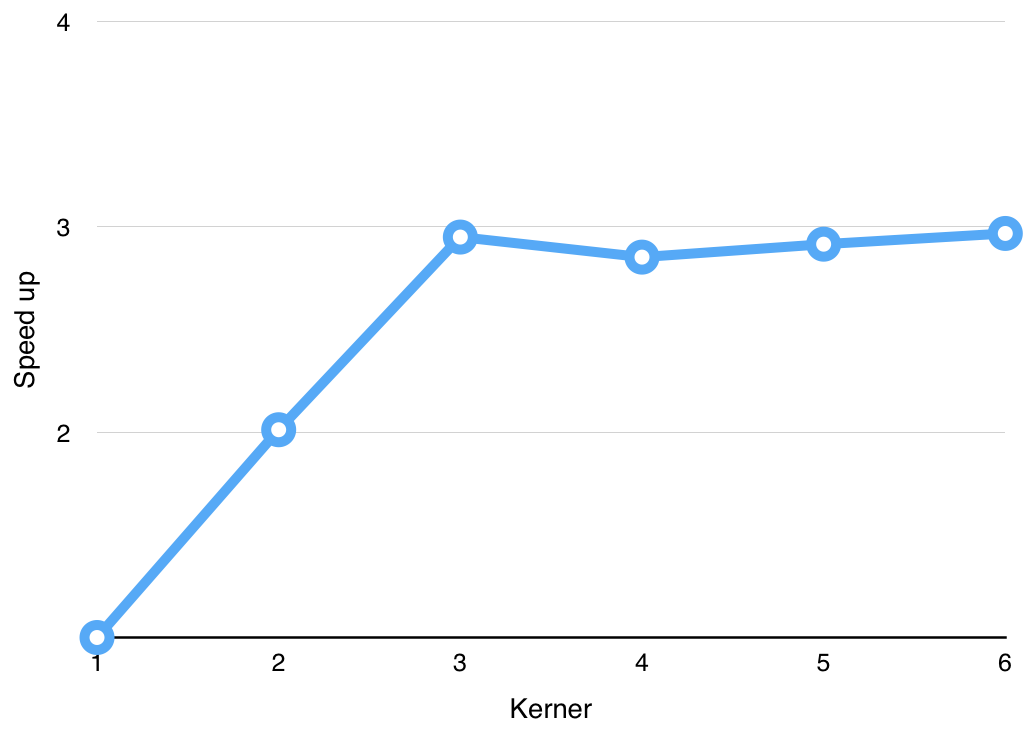
\includegraphics[width=0.95\textwidth]{graf_opg1.png}}
\caption{Graf over test resultater.}
\label{fig:opg2_2_test}
\end{figure}

\subsection{Test}
Vi testede programmet i stadier for løbende at sikre at alt fungere som det skulle. Vi foretog derfor test efter vi mente vi havde vores multitråds implementation med heltal på plads, og igen efter vi havde implementationen med kvadratrodssummering.\\

Tests af programmet blev udført ved at først benytte talsæt vi let kunne kontrollere: f.eks. skulle \textit{N} = 10 give et resultat på 55 (ved helttals summering). Ved at benytte flere eller færre tråde, og lægge til eller trække fra \textit{N} var det let at påvise hvornår programmet fungerede.\\

Det samme gjorde sig gældende for kvadratsrods summeringen, dog med andre tal. F.eks. giver \textit{N} = 9 ca. 19,306, mens \textit{N} = 8 må give et resultat præcis 3 mindre.\\

I kombination med tidstagning af store regneopgave (som tidligere nævnt) samt printlines i \textit{runner} funktionen var det muligt at demonstrere, at der blev oprettet multiple tråde, og at programmet benyttede dem til at foretage beregningerne.

\end{document}